%----------------------------------------------------------------
%
%  File    :  theory_lstm.tex
%
%  Authors : Thomas Lerchbaumer
% 
%  Created :  19 March 2022
% 
%  Changed :  19 March
% 
%----------------------------------------------------------------



\chapter{Theoretical Basis}
\label{chap:theory_basis}
As this paper aims at evaluation various NNs regarding their usage for time series forecasting this chapter explains which NNs are suitable and how they can be integrated. The knowledge of potential future bookings provide useful insights when it comes to YM. YM in general describes controlling price and capacity control in a simultaneous ways \cite{yield_m}. Therefore those predictions can be used to support bus operators in their pricing strategy. This chapter focuses on creating two prediction models utilising different techniques based on the data that is available. 
Both models are implemented using Python and the following libraries:
\begin{itemize}
\item  \verb|matplotlib|\footnote{https://matplotlib.org/} - used for plotting
\item \verb|pandas|\footnote{https://pandas.pydata.org/} - used for data manipulation 
\item \verb|tensorflow|\footnote{https://www.tensorflow.org/} - provides ML models
\item \verb|keras|\footnote{https://keras.io/} - Neural Network library
\end{itemize}

As there are various models available a literature review is conducted to figure out which models fit the purpose of time series forecasting. It turns out that the most promising NNs that can be utilised for time series prediction are either Convolutional Neural Networks (CNN) or RNN especially LSTM\cite{nn_1}\cite{nn_2}\cite{lstm_1}\cite{lstm_2}\cite{rnn_time_series_predict}.

\section{Backpropagation}
\label{sec:bp}

As both of the models LSTM and CNN use Backpropagation (BP) for its training the basic concepts of the algorithm are explained in this section. To understand the logic of BP a few terms need a detailed explanation: 
\subsubsection{Gradient}
The gradient also called gradient descent is a technique utilised to optimise the loss function used within BP. 
This implies that the gradient descent shows how the weights and biases should be changed in order to decrease the actual error value, which is the outcome of the applied loss function.
 \cite{bp_basic}
\subsubsection{Bias}
The bias is an additional parameter used in each neuron of a NN. It is used to directly influence the activation function to offset the results either to the negative or positive direction \cite{bias}. When looking at the sigmoid function without any bias in place where \verb|x| correlates to the input value and \verb|w| indicates the used weight: 
\begin{equation}
 \sigma(x) = \frac{1} {1 + e^{-{(w*x)}}}
\label{eq:eq_4}
\end{equation}
When looking at figure \ref{fig:sig_wo_bias} the weights only influence the steepness of the function but will not shift it along the x axis.
\begin{figure}[H]
	\centering
		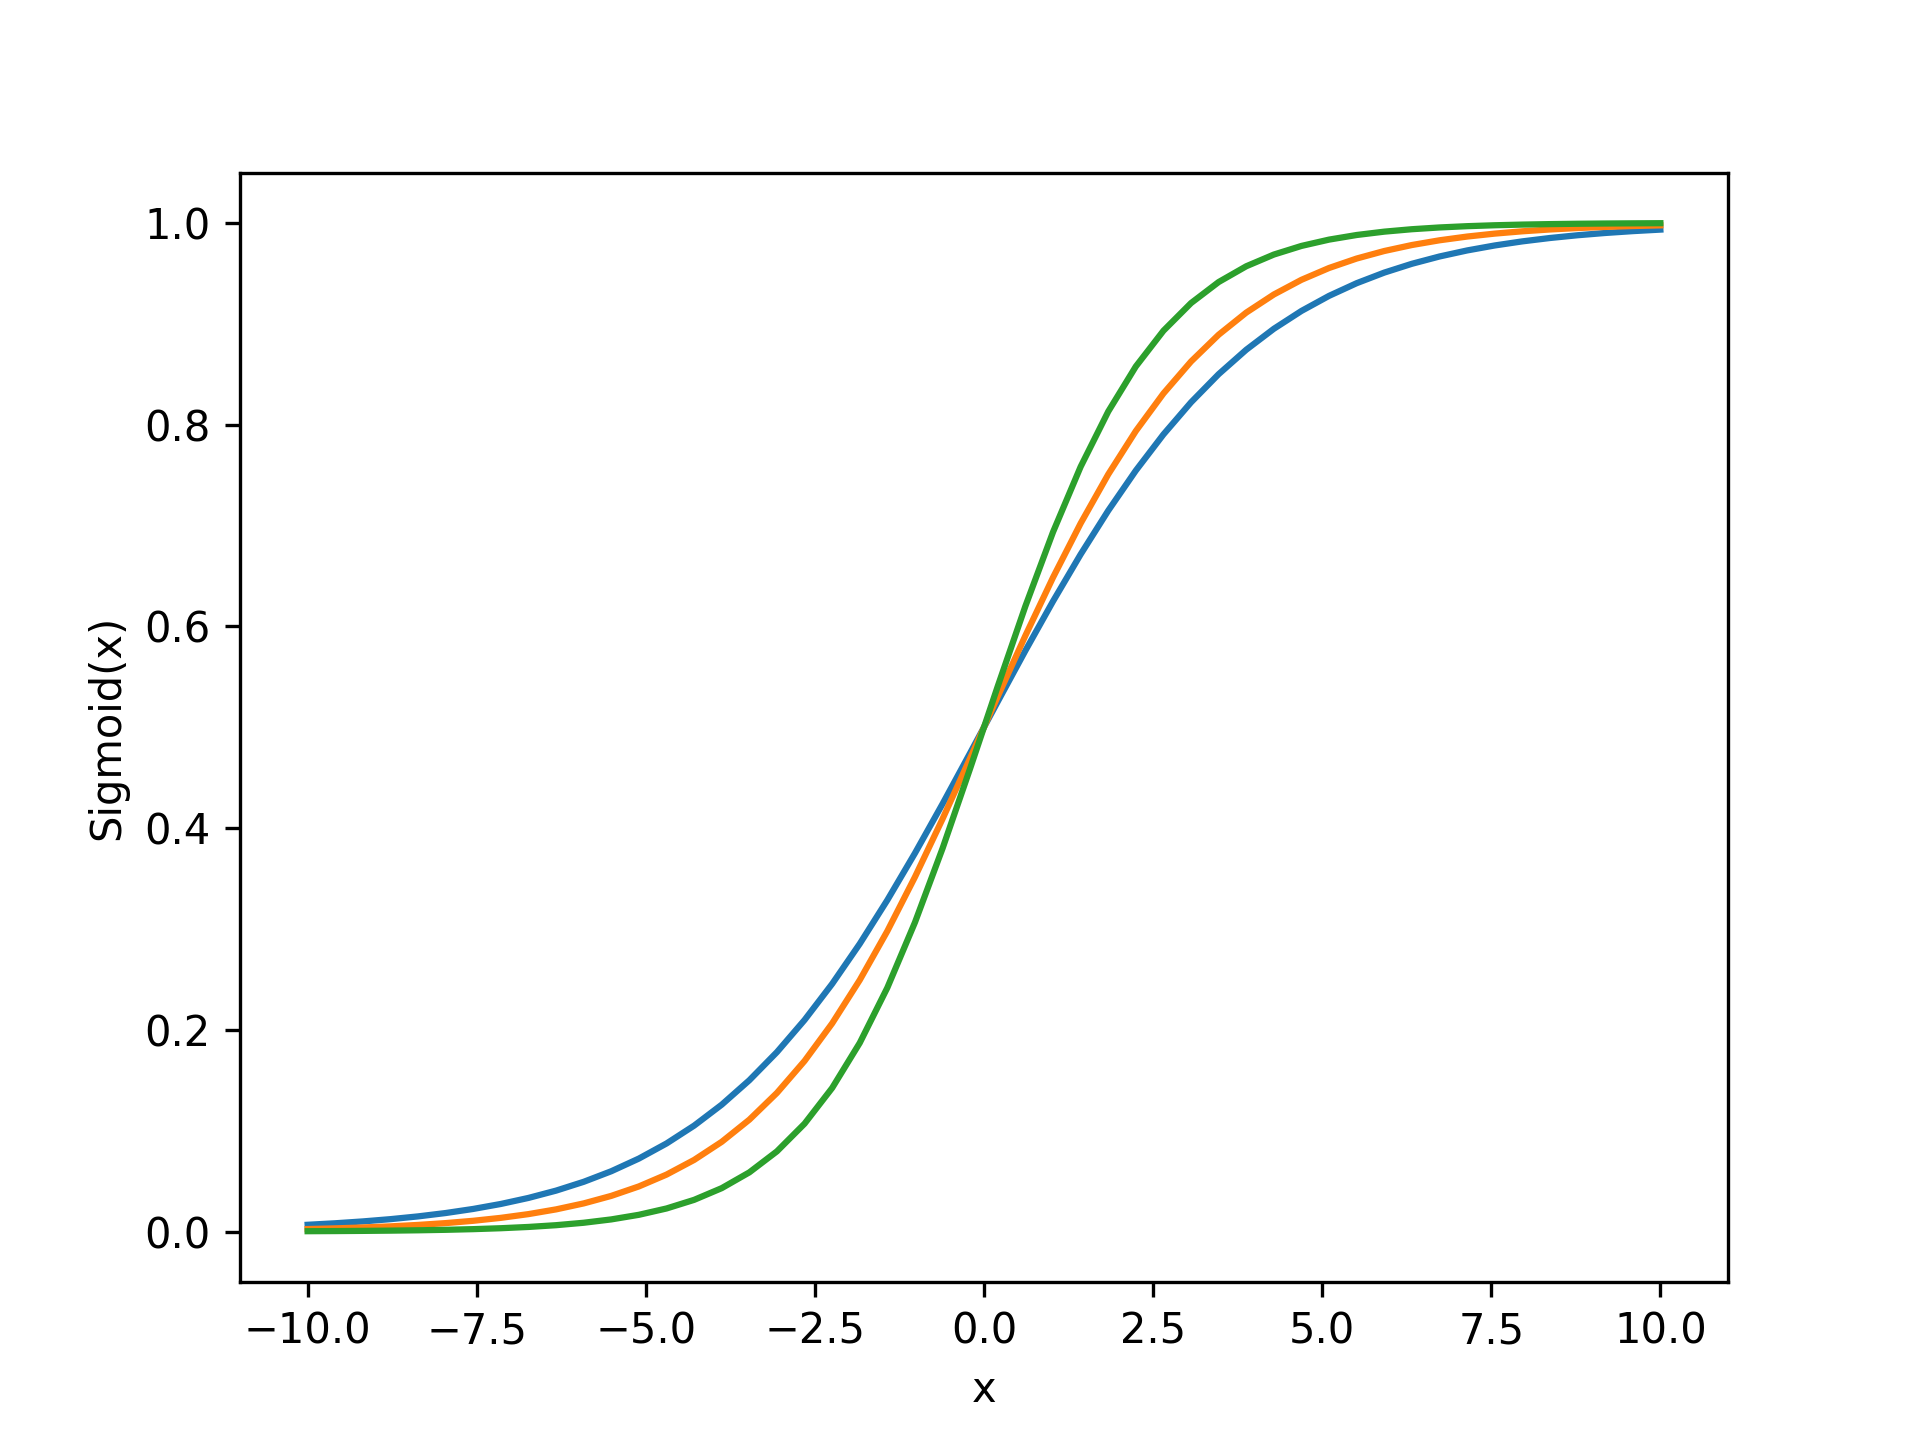
\includegraphics[width=8cm]{images/sigmoid_w_weights}
	\caption{Sigmoid function with different weights and no bias - [source:\cite{lstm_module}]}
	\label{fig:sig_wo_bias}
\end{figure}
 To shift the function along the x axis the sigmoid function is adapted with the bias \verb|b| value: 
\begin{equation}
 \sigma(x) = \frac{1} {1 + e^{-{(w*x+b)}}}
\label{eq:eq_4}
\end{equation}
By adding the bias value as constant to the sigmoid function can be shifted along the x axis as shown in figure \ref{fig:sig_w_bias}.
\begin{figure}[H]
	\centering
		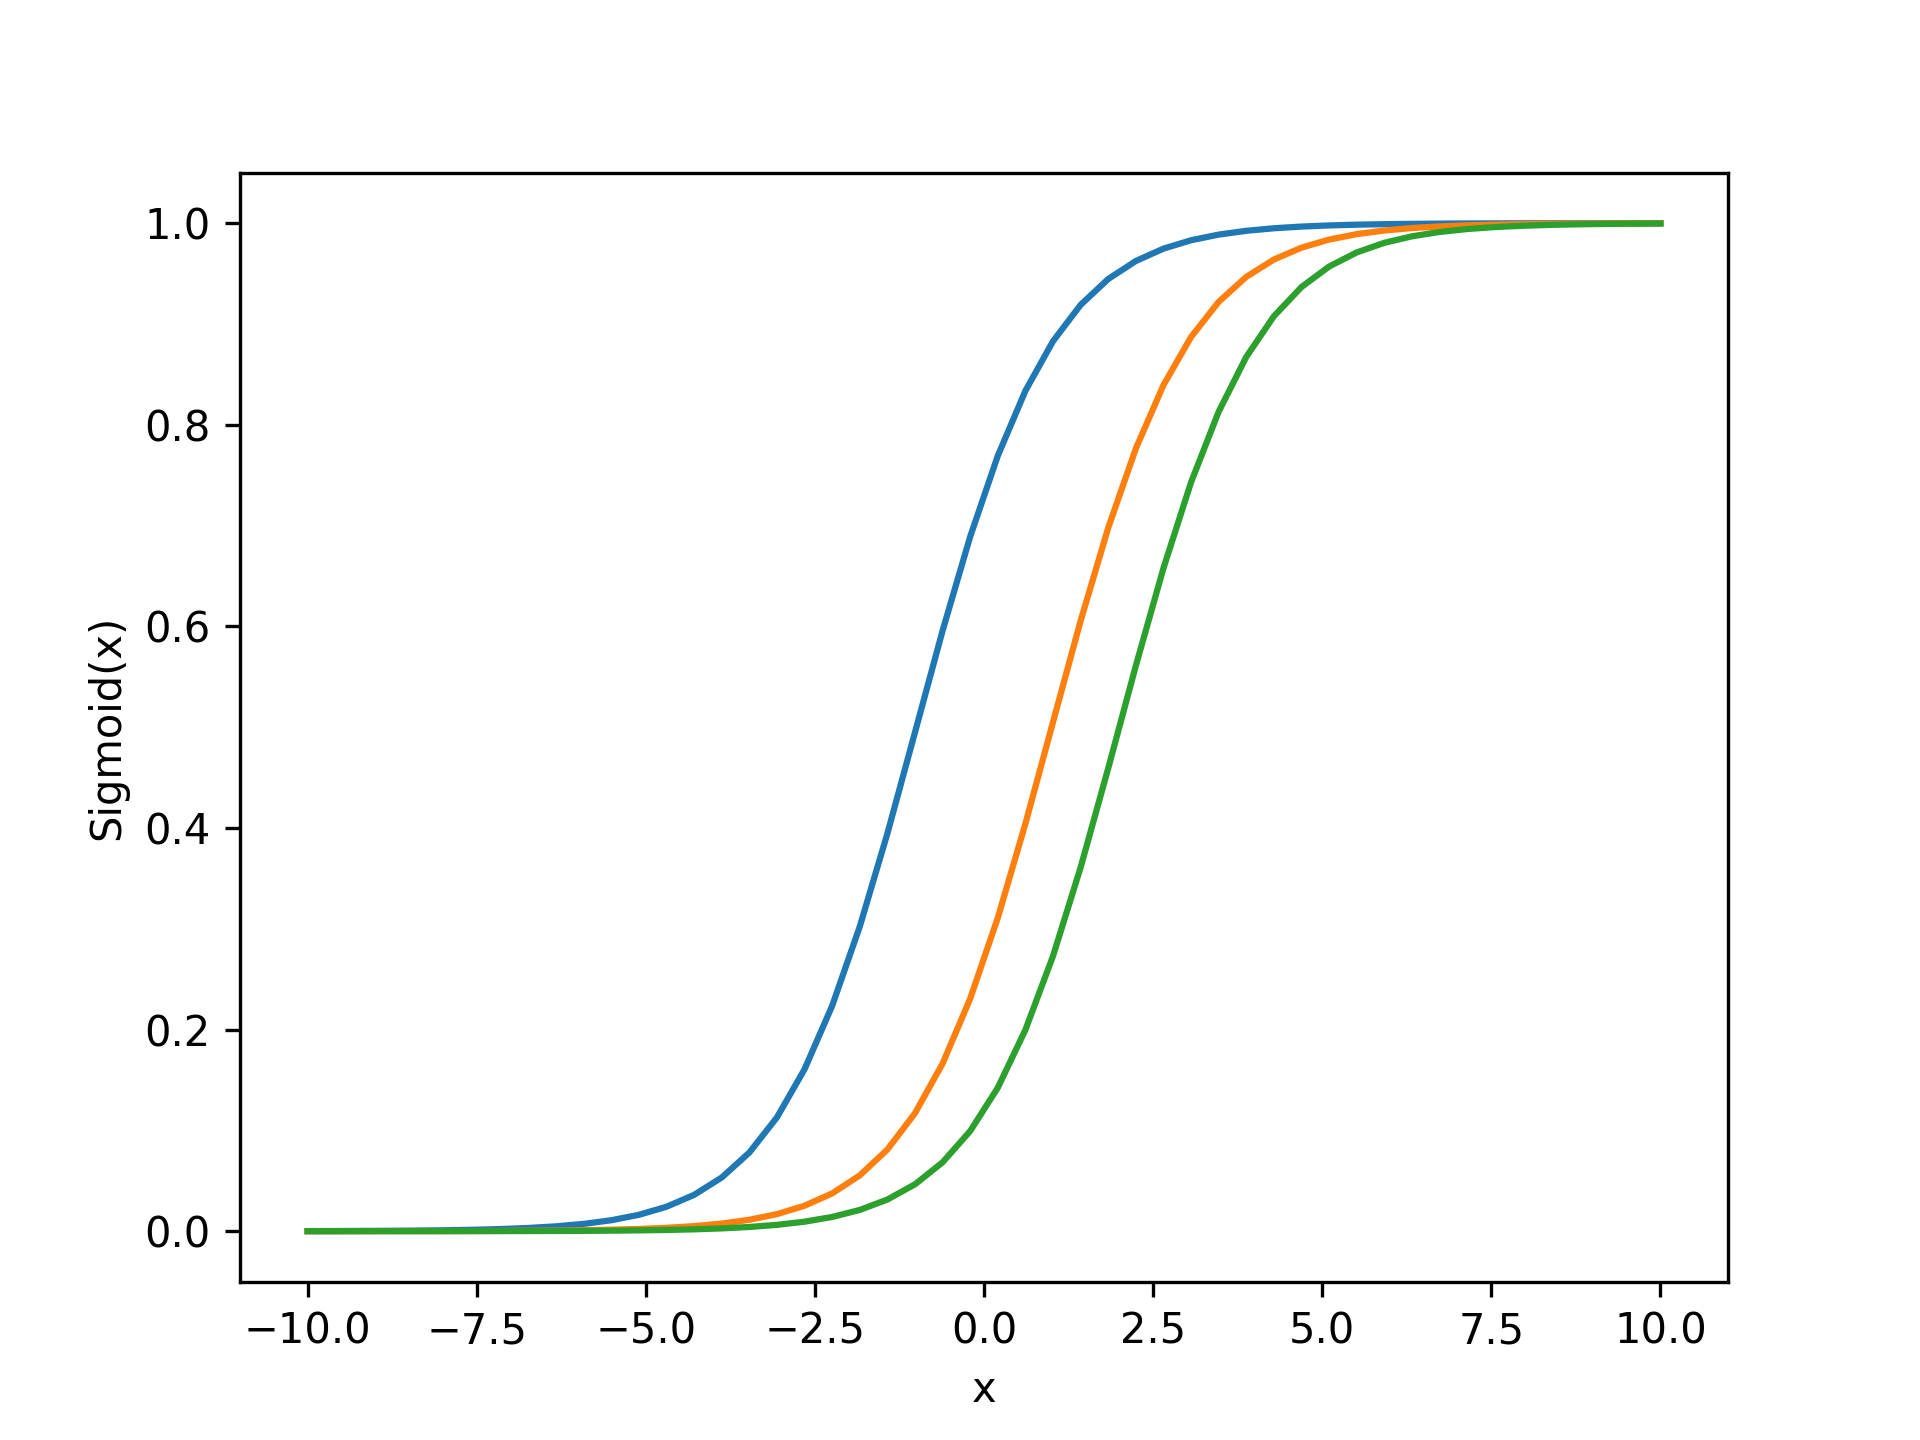
\includegraphics[width=8cm]{images/bias}
	\caption{Sigmoid function with same weights but different bias - [source:author]}
	\label{fig:sig_w_bias}
\end{figure}
The bias therefore is utilised to directly influence the result of the activation function and whether or not a certain neuron is activated or not. 
\subsubsection{Activation Function}
Activation functions introduce non-linearity characteristics to NN. This function is applied to the output of a neuron and decides whether or not a neuron is activated or not.\cite{activation} In combination with the descent gradient this function enables the NN to learn complex patterns within a training set.
The sigmoid function \cite{bp_basic} was first employed as the activation function for NN, but as of today, several additional functions, including softmax, Tanh, and ReLu, have evolved \cite{activation}.

\subsubsection{Phases} 
Backpropagation follows an iterative process. At the beginning there is the feed forward pass. During this phase the input data is passed through all layers. Each hidden layer applies a linear function to create certain weights those outputs then are fed to the activation function. The output of the activation function is utilised as the input for the following neuron, depending on how many hidden layers are employed in the NN. At the end the predicted outputs by the model are compared with the actual outputs of the training data. This comparison is evaluated through a loss function. At this step the actual learning process of the model starts by computing the gradient of the loss function based on the output of the NN. After that the back pass is initiated. Along this phase the gradients of each previous layer are multiplied with a local gradient and its weights which results in a gradient in respect to the layer's input. After receiving all gradients  based on the network's input data, all weights and biases are updated and optimised to reduce the result of the loss function. The steps forward pass, loss calculation, back pass, and the updates of weights and biases are repeated to improve the network in an iterative way. \cite{bp_basic} Figure \ref{fig:bp} demonstrates the logic of the backpropagation algorithm. Whereas \verb|wu| represents the updated weights after each iteration.  

\begin{figure}[H]
	\centering
		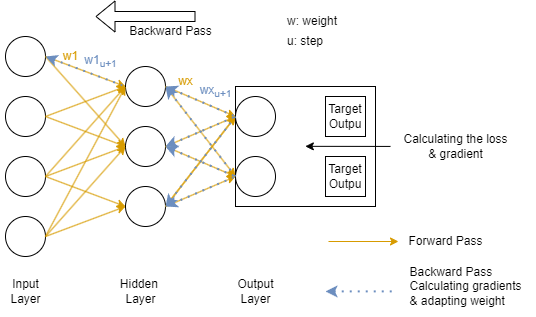
\includegraphics[width=14cm]{images/bp}
	\caption{Simplified logic of the backpropagation algorithmus - [source:\cite{bp_basic}]}
	\label{fig:bp}
\end{figure}
\section{The Models}
Time series forecasting can be performed using CNN and RNN/LSTM models. To create accurate prediction models a basic knowledge of the models functionalities are required. Therefore this section explains the components of each NN as well as the approaches those models follow. 

\subsection{LSTM}
\label{sec:lstm}
LSTM is a RNN and was invented by \cite{lstm_inventor} in 1997. Until today this NN is widley used for time series forecasting and provides reliable results for short as well as long term predictions \cite{rnn_moharm}. LSTM has so called memory cells which are responsible to store the state of data. Whenever information arrives at a memory cell its outcome is defined by refreshing the cell state with the newly arrived information. LSTM utilizes gates to control a cells state by either including or excluding information \cite{lstm_stock}. The gates are called: 
\begin{itemize}
\item input gate - data selection and storage for upcoming state
\item forget gate - data selection and storage which will not be used for the upcoming state
\item output gate - sets information within the state that is send to the output
\end{itemize}
Those gates are created by combining sigmoid functions. The results of these gates are values ranging from zero to one. A result of zero indicates the cell to not pass any information whereas values close to one indicate the cell to pass all information. 
The LSTM module or Repeating module consist of four NN layers which interact together as shown in Figure \ref{fig:lstm_rep_model}:
\begin{figure}[H]
	\centering
		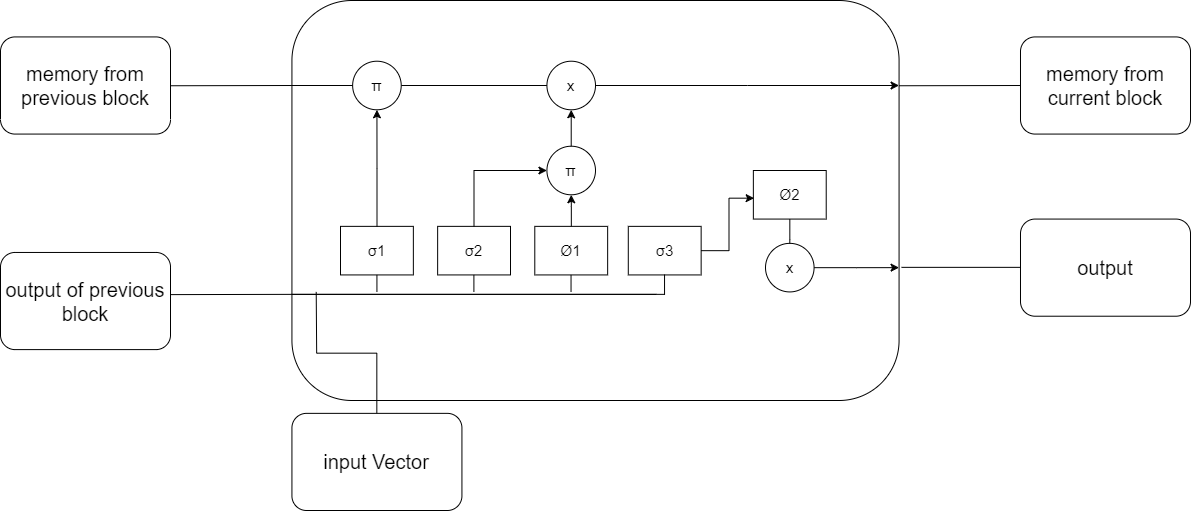
\includegraphics[width=14cm]{images/lstm_module}
	\caption{Repeating LSTM module - [source:\cite{lstm_module}]}
	\label{fig:lstm_rep_model}
\end{figure}
In total the repeating model has three gate activation functions which are named $\sigma_1$, $\sigma_2$,  $\sigma_3$ and shown in figure \ref{fig:lstm_rep_model}. Furthermore $\sigma_1$ and $\sigma_2$ act as output activation functions too. The cell state is illustrated using a blue line which starts at St-1 and indicates the previous memory block to St representing the current memory block. The amount of information that is passed is regulated by layer  $\sigma_1$ using the following function:
\begin{equation}
cf_t = \sigma_1 (W_cf * [O_t-1, x_t] + b_cf)
\cite{lstm_module}
\label{eq:eq_1}
\end{equation}
To store fresh information to the cell state, two network layers are employed. Therefore sigmoid layer $\sigma_2$ chooses the values which are updated by utilising the following formula:
\begin{equation}
l_t = \sigma_2(W_1 *[O_t-1, x_t]+ b_l)
\cite{lstm_module}
\label{eq:eq_2}
\end{equation}
Layer $\phi_1$ or \verb|tanh| is created by using new candidate values. This layer outputs a  vector by utilzing the following formular: 
\begin{equation}
\widetilde{S}_t = tanh(W_s * [O_t-1, X_t] + b_s)
\cite{lstm_module}
\label{eq:eq_3}
\end{equation}
The last step includes combination of both states \ref{eq:eq_2} and \ref{eq:eq_3} which is added to the state. Also the state is reconditioned by applying: \cite{lstm_module}
\begin{equation}
S_t = cf_t * S_t1 + I_t * \widetilde{S}_t-1
\cite{lstm_module}
\label{eq:eq_4}
\end{equation}

The reason why a LSTM model is used for this purpose is that a standalone RNN is challenging to train due to its characteristics. As BP is used for RNNs, problems like vanishing-gradient can occur. The gradient in general can be understood as a computed value through all time steps which in the end used to update parameters of the RNN. The vanishing-gradient over time results in information decay. By implementing a LSTM module this problem can be solved. \cite{lstm_overcome_rnn_problem}

\subsubsection{Bidirectional LSTM}
Bidirectional LSTMs are able to look in both directions past and future. This is achieved by processing the available data into both directions. Therefore those models make use of bidirectional layers. Those layers split up the used neurons into two directions. \cite{bi_di_1} This provides more information to the network as the model is now capable of storing the forward state as well as the backward state, resulting in potentially more accurate results \cite{bi_di_2}. 

\subsection{CNN}
\label{sec:cnn}
CNNs follow the concept of NN consisting of multiple layers. The scope of application for this kind of network reaches from computer vision problems to time-series forecast modelling. Whereas data provided for image classification is structured in multi dimensional arrays (matrices), data used for time-series forecasting is provided via one dimensional arrays.\cite{cnn_intro} A CNN provides different types of layers. Those layer types are called Pooling Layer (PL), Fully Connected (FC), Convolution layer (CL) and Flatten layer (FL). The connection of those layers are demonstrated in figure \ref{fig:cnn_struct}.
\begin{figure}[H]
	\centering
		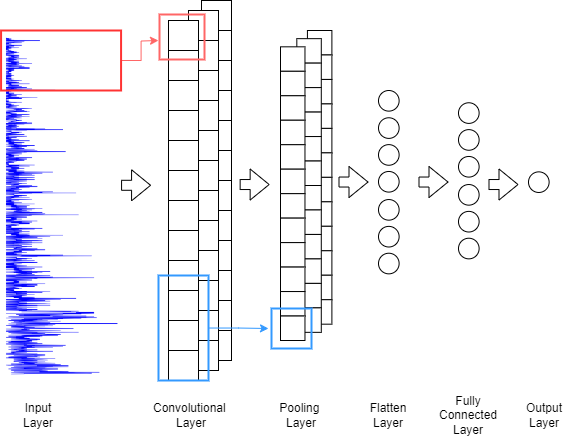
\includegraphics[width=10cm]{images/1d_cnn_model}
	\caption{One Dimensional CNN Structure - [source:\cite{cnn_vechicle}]}
	\label{fig:cnn_struct}
\end{figure}

CNN is based on convolution which is a linear operation that multiplies input data with convolution filters. Those filters which are also called kernels correlate to a set of weights \cite{cnn_vechicle}. The kernel values are created during the learning process and are optimised from the NN utilising BP. Furthermore this layer is utilised to detect features within the given one dimensional array. Those features are stored within a feature map and are calculated by applying convolutions on the input data. One crucial parameter to detect proper features is the size of the kernel. The kernel size can be understood as a number of weights that are multiplied with the input data. After each multiplication the sequence is shifted along the input data. Each shift during this process produces one output which is stored in the feature map. The following example demonstrates how this process is done:\cite{1d_cnn}
\begin{lstlisting}
Input Data: [4,7,10,43,20,10] e.g. number of bookings per day. 
Kernel: [0.5,0.25,0.2] Kernel size = 3
1st Multiplication: 4*0.5 + 7*0.25 + 10*0.2 = 5.75
2nd Multiplication: 7*0.5 + 10*0.25 + 43*0.2 = 14.6
...
Output sequence [5.75, 14.6, ...]
\end{lstlisting}
The second operation that is used within the CNN is called activation function. This non-linear function is utilised to detect complex relationships between variables and are applied onto the feature map. As of today multiple functions like ReLU, sigmoid and softmax can be used as activation functions \cite{cnn_basic3}.

The pooling layer as shown in figure \ref{fig:cnn_struct} is deployed within a NN to diminish the size of feature maps. To reduce the size pooling operations like average pooling, max pooling or sum pooling can be applied. Applying one of those operations results in less computational effort.\cite{cnn_basic}

%The activation function is also part of the fully connected layer. This layer applies the activation function onto the feature map and enables the model in combination with BP to learn complex connections between features. Furthermore this layer operates on the already flatten feature map and outputs a 2d vector.\cite{1d_cnn}

The FL converts two dimensional input data into one dimensional input vectors. Its output is used to provide values to the FC layer. Its output is used to provide values to the fully connected layer. Overfitting can be caused whenever all features are used in the flatten layer. Therefore a dropout layer can be set in place.\cite{1d_cnn} This layer cancels out neurons during the training process of a NN which reduces the model's size. 

\section{Loss Function}
\label{sec:loss_func}
The loss function is one crucial element as it evaluates the accuracy of the produced outputs from a NN. This is achieved by calculating the divergence between the predicted value and the actual value provided by the test dataset. Supervised learning deals with two different problems which is either a classification problem e.g. is the animal on the picture a cat or with regression problems like predicting future bookings. Both of those problems use a different loss function.\cite{loss_func} As this section focuses on solving a regression problem a brief overview of available loss functions and their characteristics are given. 

\begin{table*}[htbp]
	\centering
		\begin{tabularx}{\textwidth}{|l|X|}
		\hline
		\rowcolor[gray]{0.9}
		Function & Characteristics \\
		\hline
		Square loss &Sensitive to outliers (Model tends to focus on those outliers whereas accuracy for normal values decline)\\
		 \hline
		Absolute loss & Outliers do not influence the model as  severe as compared to square loss.  \\
		\hline
		Huber & Combination of square loss and absolute loss - Outliers do not influence the accuracy of results and learning from smaller errors can still be done in a efficient way  \\
		\hline
		Log-cosh & Similar to Huber when it comes to its characteristics. Does not handle large errors well because the gradient tends to stay constant. \\
		\hline
		Quantile loss & Extends absolute loss and provides prediction intervals. Utilising a punishment system for overestimated and underestimated samples. \\
		\hline
		$\epsilon$-insensitive & Focuses on samples with large prediction errors \\
		\hline	
		\end{tabularx}
	\label{tab:loss_function}
	\caption{Loss functions and their characteristics - [source:\cite{loss_func}]}
\end{table*}

By looking at the characteristics of the augmented data set shown in figure \ref{fig:augmented_data} it is clear to see that the dataset itself has got outliers repeating themselves every year. To avoid a strong focus on those peaks both models are initially trained utilising the Adam loss function.

\section{Optimise Function}
\label{sec:optimize_func}
To optimise the parameters of a NN an optimiser function is required. This function updates parameters like weights based on the results provided by the loss function \cite{optimizer}. Since both NNs described in this section make use of BP for their training. A literature review was conducted to figure out which optimiser is keen to deliver the most accurate results. By inspecting the advantages and disadvantages proposed by these works \cite{optimizer}\cite{otimizer_1}\cite{optimizer_2} it turns out that the algorithm Adam is a valid choice. This algorithm is characterised by achieving faster convergence compared to other algorithms. Furthermore Adam provides a decent performance for datasets with meager features.
Meager features can also lead to problems like underfitting and overfitting therefore those topics are discussed next. 

\section{Overfitting and Underfitting}
One problem that can occur when utilising NNs for predictions is overfitting or underfitting of the training data. Both scenarios result in a poor performance of the trained model. \cite{fitting} 
\subsection{Overfitting}

Overfitting describes the phenomenon that the model is not able to improve its problem solving capabilities after a certain period of training. There are multiple reasons for the occurrence of overfitting. One reason for example is an inaccurate or unbalanced training set. This leads to the fact that the NN produces wrong connections during its training.  Whereas the results for the training set are accurate the problems  occur during the validation phase because the model learned wrong characteristics. \cite{fitting} 
\subsection{Underfitting}
On the other hand, underfitting arises when the model cannot identify the traits of the training set and therefore struggles to achieve matching its target values. This results in high loss values. Reasons for underfitting are caused by a lack of trainable parameters as well as a NN model with a simple architecture in terms of hidden layers. \cite{fitting} 
\newline
\newline
As the data was affected during the Covid19 pandemic data augmentation which is applied during section \ref{sec:data_aug} is necessary in order to avoid both scenarios.
\newline
\newline
The basics explained during this chapter are crucial when it comes to improving a model's performance as all of the components mentioned above influence a models capability to predict future bookings. Another key element to achieve acceptable results is the utilised data itself. Therefore chapter \ref{chap:available_dataset} describes the available data, its characteristics and how the data is prepared so it can be used for time series forecasting. 
 
